\usechapterimagetrue
\chapterimage{nasa.jpg} % Chapter heading image
\chapter{Data transmission}
\usechapterimagefalse

In the previous chapter we investigated the data compression problem. That is, given a source and some noiseless means of communication, the problem is to encode the source in such a way that we minimize the usage of the noiseless communications channel while we allow the receiver to recover the message. Here we will investigate a dual problem, the problem of transmitting a source over a noisy channel. This problem, is the problem that your mobile phone faces each time that it wants to exchange information with the nearest base station. %, or the problem that your ADSL router faces to transmit information over fiber. 
It is also the same problem that your computer faces when it wants to store information on a disk in such a way that it can be recovered at a later time. %This is as we see a very relevant problem. We will not have the time to dig into great depth, but the menu should allow you to get a solid understanding of the mathematical foundations and a glimpse about how we tackle it currently. In the figure above, you can see the XXXX space XXX. As you can imagine, the bandwidth of the communications channel linking it with earth is very limited, the information we want to exchange precious and the channel rather noisy. Space exploration has been one unexpected driver of progress for pushing the limits of error correcting codes. (why error correting?)
\booksection{The communications problem}
\label{sec:comprob}
\begin{figure}[h!]
\begin{center}
\def\svgwidth{\columnwidth} 
\input{figures/shannoncom.pdf_tex}
\end{center}
\caption[Communications system diagram.]{This figure reproduces the communications system diagram introduced by Shannon~\cite{Shannon_48}.}
\label{fig:shannoncom}
\end{figure}
Let us first of all, depict the building blocks of an idealized communications problem. Our description parallels the one of Shannon~\cite{Shannon_48}, see in Fig.~\ref{fig:shannoncom} a graphical representation. The figure shows five entities: an information source, a transmitter, a noise source, a receiver, and a destination. The communications scheme works as follows: 

First the information source generates a message $m$ from a set of possible messages $M$. Then, the transmitter takes $m$ and encodes it into $n$ channel symbols. We define the coding rate $R$ as:

\begin{equation}
R=\frac{\log M}{n}
\end{equation}

%\begin{exercise}
%Suppose that we want to transmit a message from a set of $16$ messages that a source will choose uniformly at random. We have two channels available, both are noiseless, one allows to transmit one bit per channel use and we can use it once per second. The second channel allows to transmit two bits per channel use and we can use it once per minute. Over which channel can we communicate at a higher rate? How does time influence this number?
%\end{exercise}
The channel is a physical medium of transmission. Mathematically, we can model it as a system taking symbols from input alphabet $\mathcal{X}$ to symbols of output alphabet $\mathcal{Y}$ and characterized by a transition probability matrix that maps the probability of every symbol $y$ if symbol $x$ is sent. The receiver tries to undo the encoding given the noisy received signal and at the end of the scheme the destination receives the ${\hat{m}}$ possibly identical to $m$.

\booksection{Detection, correction and minimum distance}
Let us recall our original example of transmitting the weather forecast. Let us recall that the set of messages is binary : rain and sun. If we are interested in transmitting one of these messages through a noiseless channel, it should be clear that unless one of the two messages has zero probability the encoding with minimum average length will assign to rain the codeword $0$ and to sun $1$ or viceversa. 

Let us now imagine that we want to transmit the weather forecast through a noisy channel. For instance a channel that takes a binary symbol as input and outputs the same symbol with probability $1-p$ or flips it with probability $p$. In this new scenario, unless we change the encoding, the messages transmitted will be erroneous with probability $p$. The most obvious way of protecting against error is repeating the message. The repetition code of length $3$ is $C=\{000,111\}$. 

Let us suppose that we use the repetition code to encode the weather forecast, for instance $C(\text{rain})=000,C(\text{sun})=111$, we send the codeword corresponding to rain through the noisy channel described above and the channel flips the last symbol. We would receive the word 001, and we could guess that the most likely codeword corresponding to the received vector is 000. In the following we will introduce the necessary definitions to understand quantitatively this example. 

First, we introduce a distance function between vectors that will allow to justify the choice of decoding 001 to the codeword 000.
\begin{definition}
The Hamming distance between two vectors $x,y\in D^n$ is given by:
\begin{equation}
d(x,y)=|{i:x_i\neq y_i, 1\leq i\leq n}|
\end{equation}
\end{definition}
An useful way of interpreting the Hamming distance is as the minimum number of positions that it is necessary to change in $x$ to transform it to $y$.
\begin{example}
The Hamming distance between vectors $x=(1,2,0,1,2)$ and $y=(2,1,0,1,2)$ is two because they differ in the first two entries. Alternatively, from the definition
\begin{equation}
d(x,y)=|{i:x_i\neq y_i, 1\leq i\leq n}|=|{1,2}|=2
\end{equation}\end{example}
A function $d:\mathcal X\times \mathcal X\mapsto \mathbb R$ is a distance function if it verifies the following properties:
\begin{enumerate}
%\item Non-negativity: $d(x,y)\geq 0$
\item Identity: $d(x,y)=0$ if and only if $x=y$
\item Symmetry: $d(y,x)=d(x,y)$
\item Triangle inequality: $d(x,y)\leq d(x,z)+d(z,y)$
\end{enumerate}
\begin{exercise}
Show that the Hamming distance is a valid distance function
\end{exercise}
In the following whenever we refer to a distance, we will refer to the Hamming distance unless explicitly stated otherwise.

The decoding strategy that we described above is called nearest neighbor decoding or minimum distance decoding. A minimum distance decoder is a decoder that outputs the codeword closest in distance to the received vector $y$, or in the case that there are more than one it will choose from the set of closest codewords uniformly at random.
\begin{equation}
\hat x = \argmin_{x\in C}d(x,y)
\end{equation}
\begin{example}
A minimum distance decoder for the repetition code of length 3 will output 000 when it receives as input the word $001$ since $000$ has a smaller hamming distance to $001$ than the other codeword in the code: $111$.
\end{example}
\begin{definition}
A block code is a function $C:D^k\mapsto D^n$, where $D$ is a finite set and $k\geq n$ are natural numbers.
\end{definition}

%\booksection{The repetition code and two simple channels}
Let us better understand the behavior of a minimum distance decoder by analyzing how it works quantitatively. Suppose that we send each of the symbols of a codeword $x=(x_1,\ldots,x_n)$ one by one through a channel that is potentially noisy. The output will be the vector $y=(y_1,\ldots,y_n)$ with $y_i=x_i+e_i$. We can understand the role of a decoder as that of guessing the added noise vector $e=(e_1,\ldots,e_n)$ as guessing $e$ allows to undo the action of the channel.

We can now define the error rate of a word:
\begin{equation}
p_e(w)=\sum_{y\in D^n}p(y|c)p(\text{dec}(y)\neq x)
\end{equation}
and the error rate of the transmission scheme:
\begin{equation}
p_e(C)=\sum_{w\in C}p(w)p_e(w)
\end{equation}

Let us now study the effect of the repetition code in error rate on two important communications channels.

The first channel that we introduce is the binary symmetric channel. 
\begin{figure}[h]
\begin{center}
\def\svgwidth{\columnwidth} 
\input{figures/bsc.pdf_tex} 
\caption{Binary Symmetric Channel.}
\label{fig:bsc}
\end{center}
\end{figure}

\begin{exercise}
Consider $C=\{000,111\}$, suppose that we send each symbol of the word 000 through a BSC$(p)$.
\begin{itemize}
\item What is the probability of having no errors?
\item What is the probability of having one error?
\item What is the probability of having two errors?
\item What is the probability of having three errors?
\item What is the error probability with a minimum distance decoder?
\end{itemize}
\end{exercise}

\begin{figure}[h]
\begin{center}
\def\svgwidth{\columnwidth} 
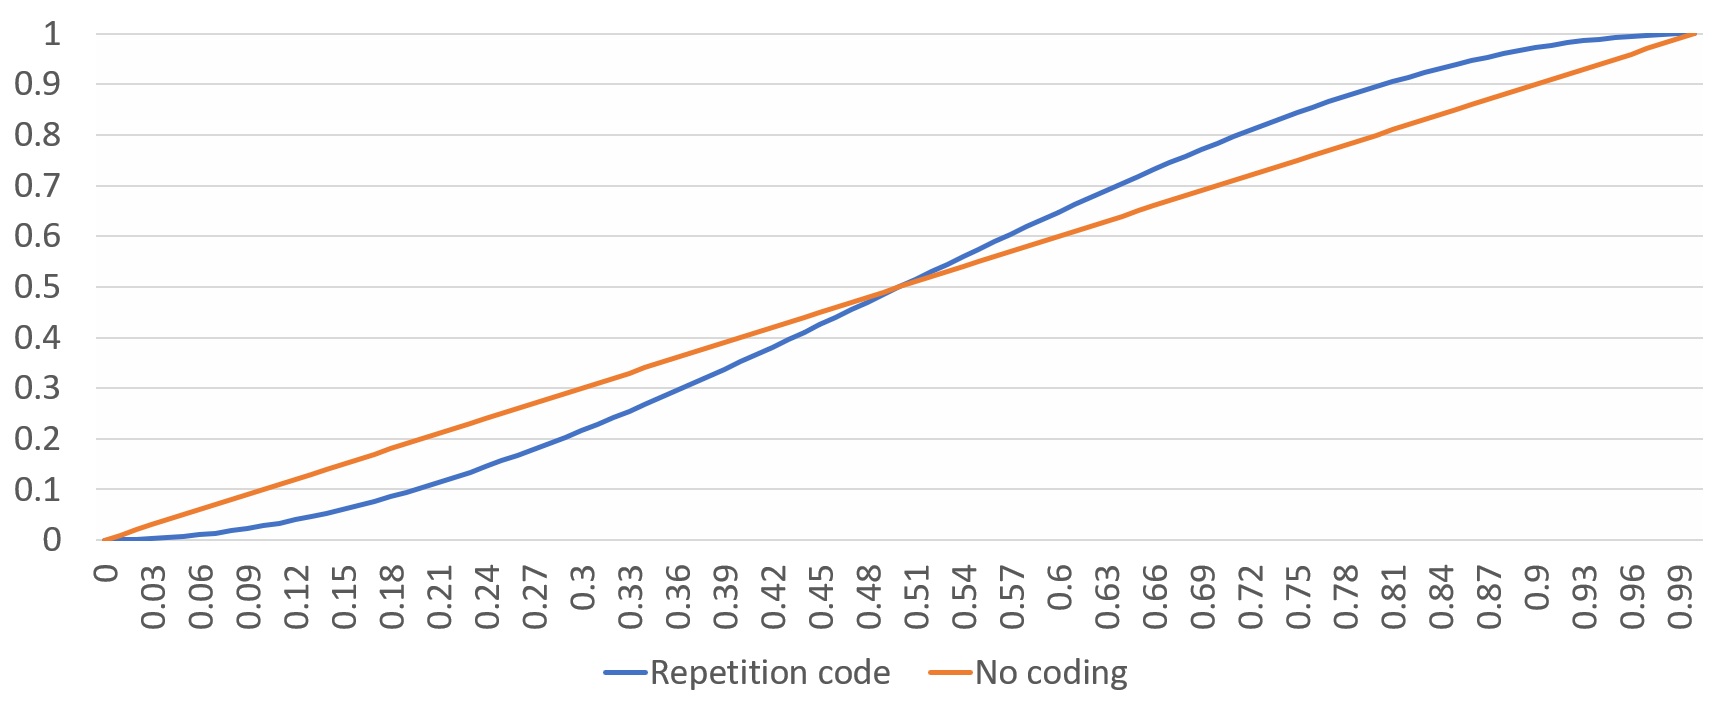
\includegraphics[width=\linewidth]{figures/bscrepcode.png} 
\caption{Decoding error vs crossover probability for the repetition code and for uncoded transmission.}
\label{fig:bscrep}
\end{center}
\end{figure}


\begin{exercise}
Consider $C=\{000,111\}$, suppose that we send each symbol of the word 000 through a BEC$(p)$.
\begin{itemize}
\item What is the probability of having no erasures?
\item What is the probability of having one erasure?
\item What is the probability of having two erasures?
\item What is the probability of having three erasures?
\item What is the error probability with a minimum distance decoder?
\end{itemize}
\end{exercise}

\begin{figure}[h]
\begin{center}
\def\svgwidth{\columnwidth} 
\input{figures/bec.pdf_tex} 
\caption{Binary Erasure Channel.}
\label{fig:bec}
\end{center}
\end{figure}

\begin{figure}[h]
\begin{center}
\def\svgwidth{\columnwidth} 
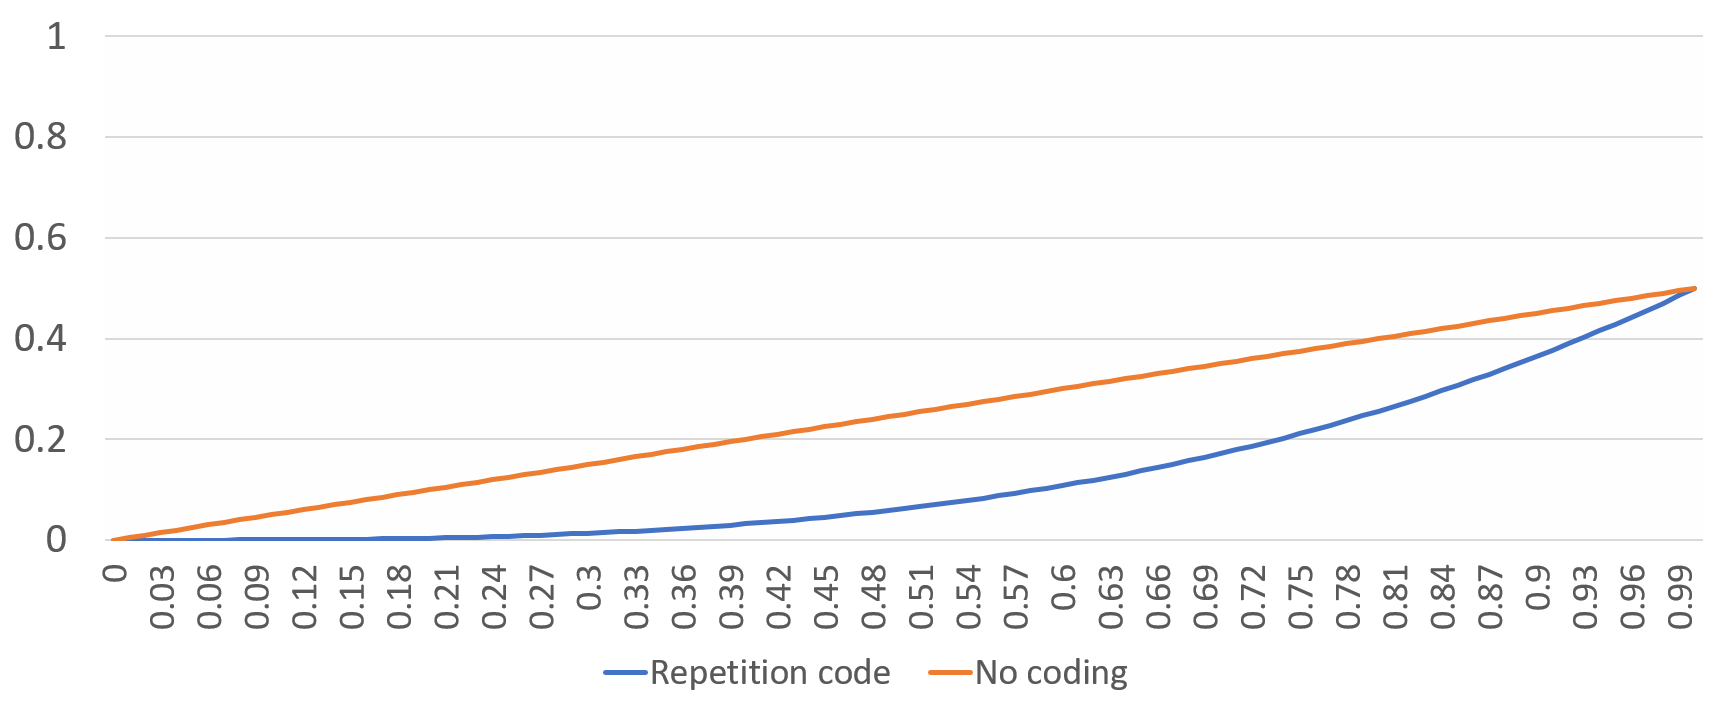
\includegraphics[width=\linewidth]{figures/becrepcode.png} 
\caption{Decoding error vs erasure probability for the repetition code and for uncoded transmission.}
\label{fig:bscrep}
\end{center}
\end{figure}

Recall that the number of strings of length n with k ones is $n\choose k$.
\begin{exercise}
Show that a code $C$ can detect all error patterns with $s$ errors if and only if $d_{\min}(C)\geq s+1$
\end{exercise}
\begin{exercise}
Show that a code $C$ can correct all error patterns with $t$ errors if and only if $d_{\min}(C)\geq 2t+1$
\end{exercise}

\begin{exercise}
Show that a code $C$ can detect all erasure patterns with $e$ errors if and only if $d_{\min}(C)\geq e+1$
\end{exercise}

\begin{exercise}
Given a code with minimum distance 12, find the maximum number of errors it can detect, the maximum number of errors it can correct and the maximum number of erasures it can correct.
\end{exercise}

\begin{definition}
An $[n,k,d]_q$ code is a code that encodes $k$ symbols from a $q$-ary alphabet into $n$ symbols of a $q$-ary alphabet and has minimum distance $n$.
\end{definition}
\begin{example}
The binary repetition code of length 3 is a $[3,1,3]_2$ code.
\end{example}

A typical coding theory problem is given two or three of the parameters in $[n,k,d]_q$ find the best code that matches those values. For instance:
\begin{itemize}
\item Given $n,k,q$ find within the set of codes encoding $k$ $q$-ary symbols into $n$, the code with the maximum minimum distance:
\begin{equation}
B_q(n,k)=\max
\end{equation}
\item Given $n,k,q$ find within the set of codes encoding $k$ $q$-ary symbols into $n$, the code with the maximum minimum distance:
\begin{equation}
A_q(n,k)=\max
\end{equation}
\item Given $n,k,q$ find within the set of codes encoding $k$ $q$-ary symbols into $n$, the code with the maximum minimum distance:
\end{itemize}
\begin{exercise}
Find $B_2(n,1)$
\end{exercise}
\begin{exercise}
Find $B_2(n,n)$
\end{exercise}
\begin{definition}
Two codes $C$ and $C'$ are equivalent if the set of codewords coincide up to a permutation in the position of the symbols, relabeling of the symbols or both.
\end{definition}
\begin{example}
The codes $C=\{001,110\}$ and $C'=\{100,011\}$ are equivalent because the codewords coincide up to a permutation of the position of the symbols.
\end{example}
\begin{example}
The codes $C=\{001,110\}$ and $C'=\{000,111\}$ are equivalent because the codewords coincide up to a relabelling of the symbols.
\end{example}

The finite field $F_2$ is the set $\{0,1\}$ together with the operations $+,\cdot$ defined as follows:
$$\begin{array}{c|cc}
+ & 0 & 1 \\
\hline
0 & 0 & 1 \\
1 & 1 & 0 
\end{array}$$
and
$$\begin{array}{c|cc}
\cdot & 0 & 1 \\
\hline
0 & 0 & 0 \\
1 & 0 & 1 
\end{array}$$
\booksection{Bounds on codes}
We will now introduce some notation about spheres on $V_n$ that will allow us to bound the possible binary codes.
\begin{definition}
Given $x\in\{0,1\}^n$, and $r\in\mathbb N$ we define the sphere of radius $r$ centered around $x$ as the set of points with distance at most $r$: $S_r(x)=\{y:d(x,y)\leq r$.
\end{definition}
\begin{exercise}
Find the set of points $S_1(x)$ with $x=(0,1,0)$.
\end{exercise}
\begin{exercise}
Let $x\in\{0,1\}^n$ and $r\in\mathbb N$, show that the number of elements in $S_r(x)$ is:
\begin{equation}
\left|S_r(x)\right|=\sum_{i=0}^rn\choose i
\end{equation}
\end{exercise}
We now have the tools to prove to important bounds for the existence of codes. The first of these bounds is called the Hamming bound, from the mathematician that proved it, but also the sphere packing bound since it argues that a code can only correct all patterns of some weight $t$ if it can fit as many spheres of radius $t$ in $V_n$ as the number of codewords.
\begin{theorem}[Hamming bound]
An $[n,k,d]$ code satisfies 
\begin{equation}
2^k\sum_{i=0}^tn\choose i\leq 2^n
\end{equation}
where $t=\lfloor\frac{d-1}{2}\rfloor$.
\end{theorem}
\begin{proof}
As shown in exercise \ref{}, a $S_t(x)$ sphere contains $\sum_{i=0}^tn\choose i$ words. For $t$ to be the maximum weight of the error patterns the code can correct it needs to be possible to place a sphere of radius $t$ around each of the $2^k$ codewords and these spheres need to be disjoint. This gives a total number of words of $2^k\sum_{i=0}^tn\choose i\leq 2^n$ which is only possible if this number is smaller than the total number of words in the space $2^n$.
\end{proof}
A code is called perfect if it attains the sphere packing bound with equality.

Now we will discuss a second bound, the Singleton bound, also based on dimensionality, but this time the argument stems from the distinguishability of codewords under erasure.
\begin{theorem}[Singleton bound]
An $[n,k,d]$-code satisfies $d\leq n-k+1$.
\end{theorem}
\begin{proof}
In a code with minimum distance $d$, if we erase $d-1$ positions of the code, all codewords need to be still different. However, the number of words of length $n-d+1$ is $2^{n-d+1}$ which can not be larger than the total number of words in the code $2^k$, i.e. $2^{n-d+1}\leq2^k$. The proof follows by taking the logarithm of both sides and solving for $d$.
\end{proof}
A code that meets the Singleton bound with equality is called maximum distance separable code.
\booksection{Refresher on linear algebra}
A vector space that is going to be very useful in the following is the $n$-dimensional binary vector space that we will denote by $V_n$. This is the vector space of length $n$ binary strings over $\mathbb F_2$. 

Addition over $V_n$ follows from addition in $\mathbb F_2$. That is, given $x,y\in\{0,1\}^n$.
\begin{equation}
x+y=(x_1+y_1,\ldots,x_n+y_n)
\end{equation}
where $x_i+y_i$ follows the rules from \eqref{}. Similarly scalar multiplication in $V_n$ follows from the multiplication rules in $\mathbb F_2$, given $s\in\{0,1\}$ and $x\in\{0,1\}^n$:
\begin{equation}
s\dot x=(s\cdot x_1,\ldots,s\cdot x_n)
\end{equation}
where $s\cdot x_i$ follows the rules from \eqref{}.
\begin{definition}
The Hamming weight $w:\{0,1\}^n\mapsto\mathbb N$ of a binary string is given by its number of ones. Given $x\in\{0,1\}^n$:
\begin{equation}
w(x)=\sum_{i=1}^nx_i
\end{equation}
\end{definition}


\begin{exercise}
Show that given $x,y\in\{0,1\}^n$, $d(x,y)=w(x+y)$.
\end{exercise}
In the following we state several important properties and definitions of vector spaces that will be of use in coding theory. Some of these, we state only for $V_n$ for simplicity. If these notions are unfamiliar or not completely understood, please review your text on the matter.

\begin{definition}
$U$ is a subspace of $V$ if $U\subseteq V$ and $U$ is a vector space.
\end{definition}
\begin{example}
$\{000,111\}$ is subspace of $V_3$.
\end{example}
\begin{definition}
A linear combination of the vectors $v^1,v^2,\ldots,v^n\in \{0,1\}^n$ is a vector $s_1\cdot v^1+s_2\cdot v^2+\ldots+s_n\cdot v^n$ where $s_1,s_2,\ldots,s_n\in\mathbb F_2$.
\end{definition}
\begin{example}
$0\cdot(0,0,1)+1\cdot(1,1,0)=(1,1,0)$ is a linear combination of the vectors $(0,0,1)$ and $(1,1,0)$.
\end{example}
\begin{definition}
The set of linear combinations of a set of vectors is called its span.
\end{definition}
\begin{exercise}
Show that the span of a set of vectors is a vector space.
\end{exercise}
\begin{definition}
A set of vectors $v^1,v^2,\ldots,v^k\in \{0,1\}^n$ is linearly dependent if there exist $s_1,s_2,\ldots,s_k\in\{0,1\}^k$ different from $0,\ldots 0$ such that $s_1\cdot v^1+s_2\cdot v^2+\ldots+s_n\cdot v^n=0$.
\end{definition}
\begin{definition}
A set of vectors $v^1,v^2,\ldots,v^k\in \{0,1\}^n$ is linearly independent if the  $s_1,s_2,\ldots,s_k\in\{0,1\}^k$ different from $0,\ldots 0$ such that $s_1\cdot v^1+s_2\cdot v^2+\ldots+s_n\cdot v^n=0$.
\end{definition}
\booksection{Binary linear codes}
A binary linear code of length $n$ is a subspace of $V_n$.
\begin{exercise}
Show that the repetition code of length 3 is a subspace of $V_3$.
\end{exercise}
\begin{exercise}
If $C$ is a binary linear code then:
\begin{equation}
\min_{x,y\in C}d(x,y)=\min_{x\in C\setminus\{0\}}w(x)
\end{equation}
\end{exercise}
\begin{definition}
Given a $[n,k,d]$ linear code, a matrix with $k$ rows and $n$ columns where each row is an element of a basis of the code is called a generator matrix.
\end{definition}
\begin{example}
A generator matrix for the length three repetition code is given by:
\begin{equation}
\begin{pmatrix}[ccc]
1 & 1 & 1
\end{pmatrix}
\end{equation}
\end{example}
\begin{exercise}
Two generator matrices $G_1,G_2$ with coefficients in $\{0,1\}$ generate two equivalent binary codes if it is possible to transform $G_1$ into $G_2$ by a series of row permutations, column permutations and additions of one row into another.
\end{exercise}
\begin{lemma}
Any generator matrix $G$ of an $[n,k,d]$ binary linear code can transformed to a generator matrix of the form $G'=\left(I_k|A\right)$ where $I_k$ is the $d$-dimensional identity matrix and $A$ is an arbitrary $n-k\times k$ matrix. This matrix form is called \textit{standard form}.
\end{lemma}
\begin{exercise}
Take the following generator matrix to standard form:
\begin{equation}
G=\begin{pmatrix}[ccccc]
0 & 1 &0 &0 &1\\
1 & 1& 0 & 0 &\\
0 & 0 & 1  &0 & 0
\end{pmatrix}
\end{equation}
\end{exercise}
%\iffalse
We define $C$, the capacity of a channel, as the maximum mutual information over all possible input distributions: 

\begin{eqnarray}
\label{eq:capform}
C = \max_{p(x)} I(X;Y)
\end{eqnarray}

\booksection{Converse theorem for noisy channel coding}
The converse statement follows from Fano's inequality \cite{Fano_61}. The intuition behind this part is that if we think of an encoding that achieves a vanishing error probability, then necessarily $R<I(X;Y)$~\cite{Cover_91}. 

The past sections have been devoted to schemes that achieve a compression rate slightly larger than the entropy. We have called these schemes optimal. We also discussed that codes that have no error have an average length bounded from below by the entropy. In this section we will investigate what happens if we can tolerate some error. Surprisingly, we can not do much better than entropy. 

Let us first introduce Fano's inequality as it will be the main tool in our argument. Suppose that we want to guess the value of random variable $X$ and we have access to random variable $Y$, let us call $\hat X=g(Y)$ the random variable that characterizes the guess. We denote by $E$ the random variable that takes value 1 if $X=\hat X$ and 0 when $X\neq\hat X$. we can now state Fano's inequality:
\begin{theorem}[Fano's inequality]
Let $X,Y$ be two random variables and $\hat X=g(Y)$ for some function $g:\mathcal Y\mapsto\mathcal X$ and let $E=I(X=\hat X)$. Then:
\begin{equation}
H(X|Y)\leq H(E) + p_E(E=1)\log(|\mathcal X -1|)
\end{equation}
\end{theorem}
\begin{proof}
Let us first expand $H(X,E|Y)$ in two different ways applying the chain rule. First:
\begin{align}
H(E,X|Y) &= H(E|Y)+H(X|E,Y)\\
         &\leq H(E) + H(X|E,Y)\\
         &= H(E) + p_E(0) H(X|E=0, Y) + p_E(1)H(X|E=1,Y)\\
         &= H(E) + p_E(1)H(X|E=1,Y)\\
         &\leq H(E) + p_E(1)\log(|\mathcal X|-1)
\end{align}
where the first equality follows from the chain rule, the first inequality since conditioning reduces entropy, the second equality follows from application of the definition of conditional entropy and the second one since in the event that the error is zero, there is no uncertainty on the value of $X$, the last inequality follows since entropy can never be larger than the logarithm of the number of outcomes.

Let us note that $H(E,X|Y)$ can also be expanded as:
\begin{align}
H(E,X|Y)&=H(X|Y)+H(E|X,Y)\\
        &=H(X|Y)
\end{align}
where the first equality follows from the chain rule and the second because if both $X$ and $Y$ are known, then $E$ is also known.

The proof ends by joining \eqref{} with \eqref{}
\end{proof}
\begin{exercise}
In \eqref{}, we have that $H(X|E=1,Y)\leq \log(|\mathcal X|-1)$. Why can we remove one outcome from the alphabet of $X$?
\end{exercise}
\booksection{Hamming codes}

%\booksection{Random codes}
\booksection{Sketch of the noisy channel theorem}

The capacity of a channel specifies the maximum rate at which a source can be reliably sent through a channel. On the other hand, no source with a rate over the capacity of the channel can be sent with a vanishing error probability.

\begin{figure}
\begin{center}
\def\svgwidth{\columnwidth} 
\input{figures/channel.pdf_tex} 
\caption[Jointly typical sequences]{Graphical representation of the input and output typical sequences. A good encoding chooses as codewords a subset of the input typical sequences that produces disjoint sets of output typical sequences.}
\label{fig:channel}
\end{center}
\end{figure}

A sketch of the proof would be as follows. Encoder and decoder share a code-book of $2^{nR}$ codewords chosen within the $2^{nH(X)}$ typical sequences~\cite{Massey_77}. The encoder sends a codeword ${x}$ drawn with uniform probability. The decoder outputs a word $\hat{{x}}$ jointly typical with the received word ${y}$. It declares an error if ${x}$, ${y}$ are not jointly typical and a decoding error can occur if there exists ${x}'\neq {x}$ jointly typical with ${y}$. We know by Eq.~\ref{eq:jointtypical} that the probability of non-joint typicality for long enough $n$ can be made as small as desired. %We can bound the second source of error $p_e$ as well:

%\begin{eqnarray}
%p_e &\leq&  \left( 2^{nR}-1 \right) \frac{2^{n(H({XY})-\delta )}}{2^{n(H(X)-\delta )}2^{n(H(Y)-\delta )}}\nonumber\\
%     &\leq & 2^{-n(I(X;Y)-R-3\delta)}
%\end{eqnarray}
%\noindent in the first inequality we have bounded the error probability as the probability that one among the $2^{nR-1}$ remaining codewords belongs to the set of jointly typical sequences. The error probability vanishes only if $R<I(X;Y)$. However, we did not impose any condition on the $p(x)$ in the above discussion. In other words, if we choose the distribution that maximizes $I(X;Y)$, the typical sequence encoding achieves the capacity of the channel.

The intuition behind the achievability proof is simple. The decoder has access to two sets: the set of sequences jointly typical with ${y}$, and the set of codewords. If the intersection is to be a single word, every codeword has to be jointly typical with a disjoint set of typical output words. 

Approximately, every codeword is jointly typical with $2^{nH(Y|X)}$ words. Then the number of jointly typical output words with input codewords is upper bounded by $2^{nR+nH(Y|X)}$, where $R$ is the coding rate. This number should be much smaller than the total number of typical sequences $2^{nH(Y)}$:
 
\begin{equation*}
2^{nR+nH(Y|X)} < 2^{nH(Y)}
\end{equation*}

\noindent which operating returns the expected result:

\begin{equation*}
R < I(X;Y)
\end{equation*}

In conclusion, as long as the coding rate is below the mutual information between input and output for $n$ long enough we can construct a code that allows the decoder to distinguish between codewords with a vanishing probability of error.

\booksection{The capacity of some basic channels}

%\subsection{Binary Symmetric Channel}
In the {BSC} the binary elements or bits are either perfectly transmitted with probability $1-p$ or flipped with probability $p$. 

Let us first find the mutual information between the input $X$ and the output $Y$~\cite{Cover_91}::

\begin{eqnarray}
I(X;Y) &=& H(Y) - H(Y|X) \\
         &=& H(Y) - \sum_x p(x)H(Y|x) \\
         &=& H(Y) - \sum_x p(x)H(p,1-p) \\
         &=& H(Y) - H(p,1-p)\sum_x p(x) \\
         &\leq & 1 - H(p,1-p)\label{eq:bscC} 
\end{eqnarray}

We obtain the capacity by finding the maximum of the mutual information for all possible input distributions. It can be easily verified that the the uniform distribution reaches the upper bound in Eq.~\ref{eq:bscC} and the capacity of the {BSC} is one minus the binary entropy of $p$.
%and this capacity is achieved for $p(X=0)=p(X=1)=\frac{1}{2}$.
%\end{proof}

%\subsection{Binary Erasure Channel}
The {BEC} was introduced by Elias in his famous paper "Coding for Two Noisy Channels"~\cite{Elias_55}. The {BEC} has two input elements while the output alphabet is composed of three elements: 0, 1, and $e$, which stands for an erasure in the channel. In this channel the bits are either correctly transmitted with probability $1-p$, or are erased with probability $p$. 

We can first find $H(X|Y) $: 

%\begin{proof}

%\begin{eqnarray}
%\label{eq:beccap1}
%H(Y) &=& H((1-p )(1-\pi ),p , (1-p ) \pi) \\
%        &=&  H(1-p , p ) + (1-p ) H(\pi, 1 - \pi )
%\end{eqnarray}
%\begin{eqnarray}
%\label{eq:beccap2}
%H(Y|X) &=& (1 -\pi )H(p, 1-p ) + \pi H(p, 1- p) \\
%           &=& H(p, 1- p)
%\end{eqnarray}
\begin{eqnarray}
\label{eq:beccap}
H(X|Y) &=& \pi (1-p )H(X|Y=0) \nonumber\\
           && + \left( \pi\, p +(1-\pi)p\right) H(X|Y=e)\nonumber\\
           && + (1-\pi)(1-p)H(X|Y=1) \\
           &=& p
\end{eqnarray}
\noindent where $p(X=0)=\pi$.The second equality holds from $H(X|Y=1)=H(X|Y=0)=0$ and $H(X|Y=e)=1$. We can now plug Eq.~\ref{eq:beccap} in Eq.~\ref{eq:mutualinformation} and bound from above the mutual information:
\begin{eqnarray}
I(X;Y) &=& H(X) - H(X|Y) \\
         &=& H(\pi, 1-\pi) - p\\
         & \leq & 1 - p\label{eq:becineq}
\end{eqnarray}
\noindent equality in Eq.~\ref{eq:becineq} is achieved again by the uniform distribution. That is, for $\pi=\frac{1}{2}$.
%\end{proof}
%\begin{eqnarray}
%C = \max_{p(x)} I(X;Y) = 
%\end{eqnarray}

It might seem that the capacity of a {BSC} that flips bits with probability $p$ is greater than the capacity of a {BEC} that erases bits with probability $p$. Fig.~\ref{fig:becbsc} shows that it is the opposite situation. On the range $p\in\left( 0,0.5\right)$, the capacity of the {BEC} is greater than the capacity of the {BSC}. Bits on the {BEC} are either perfectly known or perfectly unknown, however, it is not possible to distinguished flipped bits from correct bits in the {BSC}.

\begin{figure}[h]
\begin{center}
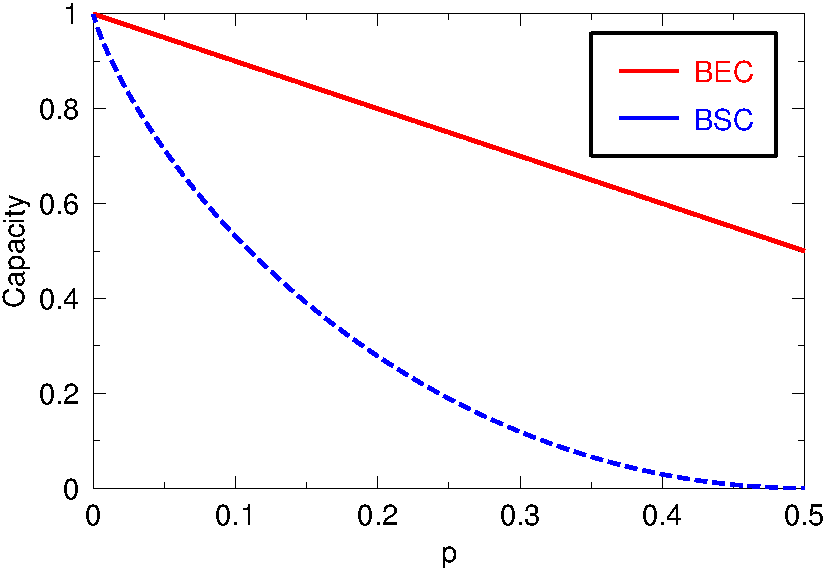
\includegraphics[width=\linewidth]{figures/becbsc.pdf}
\caption{The capacity of the BEC and BSC.}
\label{fig:becbsc}
\end{center}
\end{figure}
%\fi
\booksection{Exercises}
\iffalse
\begin{exercise}
Let $C$ be a linear binary code. Prove that either all codewords have even Hamming weight or half of the codewords have even weight and half odd weight.
\end{exercise}
\fi

\booksection{Further reading}
Chapter 7 in \cite{Cover_91}. 
